\subsection{Problem Area}
IoT has seen a rapid growth over the last few years. According to IoT Analytics the total number of IoT devices is set to surpass the total number of other connected devices around 2021 \cite{StateofIoT:online}. Further, most IoT devices will be used in WPAN \footnote{Wireless Private Area Networks includes technologies like Zigbee,Z-wave and Bluteooth} and WLAN\footnote{Wireless Local Area Networks includes mainly Wi-Fi}. 
% In contrast to 5G, these technologies don't connect to an access point from an Internet provider but rather require another user operated device to connect to the Internet, a so called "gateway"
Traditionally these devices connect to the enterprise or service provider core networks through a gateway. This gateway was mainly a router operating at L3\footnote{L3 stands for Layer 3, the networking layer in the OSI model.} to route packets and translate between different types of network protocols. \cite{lee2017futureOfIoT}. However, according to Dejan Bosanac, a senior software engineer at Red Hat in the field of cloud messaging and IoT platforms, due to their proximity to the sensors and the end user, these devices have three main advantages over the cloud: "Low latency, availability and locality"
 \cite{Introducing:kubeedge}.
 Because of this advantage system designers started to construct hybrid systems, in which the gateway plays an active role in the data processing pipeline. This architectural style of carrying out substantial amount of computation and storage at the edge is called "fog computing" \cite{fogComputing:def} and a simple example can be seen in \cref{fig:iotDeviceSetup}. 
 \begin{figure}[h!]
     \centering
     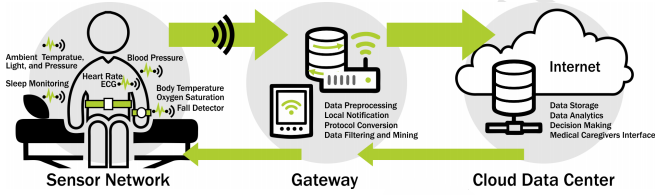
\includegraphics[scale=1.8]{figures/iotSetup.png}
     \caption{IoT Device Setup \cite{iotGatewaySlavesGraph}.}
     \label{fig:iotDeviceSetup}
 \end{figure}\\

But fog computing does not come without its drawbacks. Depending on the protocol edge devices need to be close to their peers and slaves and physically accessible for maintenance. Which also poses a major security risk as they could be accessed by malicious intruders. The software maintenance is another critical aspects. Often IoT and edge devices are not update and patched with critical consequences. The "2016 Dyn cyberattack" used IoT devices like residential gateways, smart fridges, baby phones ect. to bring down the DNS-Servers operated by Dyn making large part of the Internet unaccessible for hours\cite{dynAttack}. The authors also stress that "large number of IoT devices are accessible over public Internet" and that "security (if considered at all) is often an afterthought in the architecture of many wide spread IoT devices"\cite{dynAttack}.\\
The question is then, how can manage and secure those devices. In this report, I will solely be concerned with the software aspect, which can mitigate some effects of exposing physical hardware to more accessible places.\\
Many challenges facing edge devices today have already been solved, although in a slight different context: The cloud\cite{Introducing:kubeedge}. In the cloud 




% Note: Maybe make a graph cloud setup, user connecting to nodes, VS fog computing, sensors and users connecting to gateways and gateway to cloud.  https://www.einfochips.com/blog/iot-gateways-drivers-for-fog-computing/